\documentclass[11pt,a4paper]{article}

\usepackage[margin=1in, paperwidth=8.3in, paperheight=11.7in]{geometry}
\usepackage{amsmath,amsfonts,fancyhdr,bbm,graphicx,tikz}
\usetikzlibrary{automata,positioning}
\graphicspath{ {img/} }
\usepackage[section,nohyphen]{DomH}
\headertitle{Applied Deep Learning - Notes}

\begin{document}

\title{Applied Deep Learning - Notes}
\author{Dom Hutchinson}
\date{\today}
\maketitle

\tableofcontents\newpage

\section{Machine Learning}

\begin{definition}{Deep Representation Learning}
  \textit{Representation Learning} is a set of techniques in machine learning where a system can automatically learn representations needed for feature detection from the raw data without the need for hand-designed feature descriptions. \textit{Deep Representation Learning} is then learning to classify using this feature detection.
\end{definition}

\section{Artificial Neural Networks}

\begin{remark}{Biological Inspiration}
  In the natural world \textit{Neurons} are the basic working units of the brain. \textit{Neurons} can be split into three main areas
  \begin{enumerate}
    \item \textit{Dendrites} - Receives inputs from other neurons.
    \item \textit{Axon} - Carries information.
    \item \textit{Axon Terminals \& Synapses} = Send information to other neurons.
  \end{enumerate}
  \textit{Artificial Neural Networks} seek to mimic this structure.
\end{remark}

\begin{definition}{Neuro-Plasticity}
  \textit{Neuro-Plasticity} is the ability of a neural system to adapt its structure to accommodate new information (i.e. Learn). This can take several forms including growth \& function changes.
\end{definition}

\begin{definition}{Feed-Forward Network} is an artificial neural network where the connections between nodes are uni-directional. Data is provided to the input layer and then an output is returned from the output layer, no layers are visited twice.
\end{definition}

\begin{proposition}{Neural Networks as an Ensemble of Sub-Networks}
  A \textit{Neural Network} can be considered to represent many \textit{sub-networks}. These sub-networks are switched between depending on which components are picked and how they are defined.
  \begin{center}
    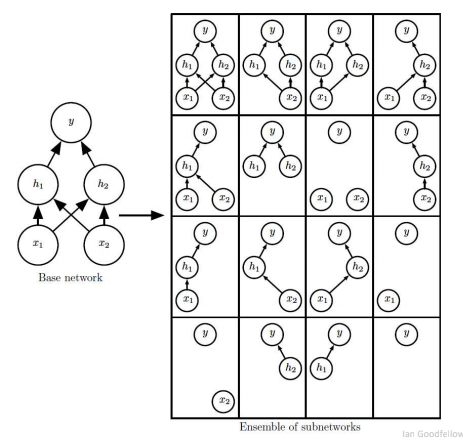
\includegraphics[width=.35\textwidth]{SubNeuralNetworks.PNG}
  \end{center}
\end{proposition}

\subsection{Perceptron}

\begin{definition}{Perceptron}
  A \textit{Perceptron} is an algorithm for supervised learning of a binary classifier. A perceptron defines a hyperplane which acts as a decision boundary which linearly separates the input-state space. These two regions correspond to the two-classes. A perceptron has the following structure.

  \begin{center}\begin{tikzpicture}
    % nodes
    \node         at (-2,0)      {$\text{bias}\big\{$};
    \node[circle] at (0,0)  (x0) {$x_0:=-1$};
    \node[circle] at (0,-1) (x1) {$x_1$};
    \node[circle] at (0,-2) (x2) {$x_2$};
    \node         at (0,-3) (x3) {$\vdots$};
    \node[circle] at (0,-4) (xk) {$x_k$};
    \node         at (0,1)       {$\overbrace{}^{\text{input}}$};

    \node[rectangle] at (3,-2) (sum) {\huge $\Sigma$};
    \node            at (3,1)       {$\overbrace{}^{\text{weighted sum}}$};
    \node[rectangle] at (6,-2) (act) {\huge $g$};
    \node            at (6,1)       {$\overbrace{}^{\text{activation function}}$};
    \node[rectangle] at (9,-2) (out) {\huge $y\in\{-1,1\}$};
    \node            at (9,1)       {$\overbrace{}^{\text{output}}$};

    % edges
    \path[->]
    (x0) edge node[above] {$w_0$} (sum)
    (x1) edge node[above] {$w_1$} (sum)
    (x2) edge node[above] {$w_2$} (sum)
    (x3) edge (sum)
    (xk) edge node[above] {$w_k$} (sum)
    (sum) edge (act)
    (act) edge (out);
  \end{tikzpicture}\end{center}
  \begin{itemize}
    \item[$x_0$] is the bias element. It is always set to $-1$ in the input and the actual value is defined by its weight $w_0$.
    \item[$\pmb{x}=(x_0,\dots,x_k)$] is the input. $(x_1,\dots,x_k)$ are the inputs for the item we wish to classify
    \item[$\pmb{w}=(w_0,\dots,w_k)$] is the weights assigned to each input.
    \item[$\Sigma$] is the weighted sum of the bias \& inputs. $\Sigma:=(\sum_{i=0}^kw_ix_i)=\pmb{w}^T\pmb{x}$
    \item[$g$] is the \textit{Activation function} which maps from $\Sigma$ to $\{-1,1\}$, effectively performing a binary classification. The user has several options for how to define this. (n.b. $g:\reals\to\{-1,1\}$)
    \item[$y$] is the output of the \textit{Activation function}. (i.e. the classification). Typically denoted as $f(\pmb{x};\pmb{w})$ \[ y=g\left(\sum_{i=0}^kx_iw_i)\right)=g(\pmb{w}^T\pmb{x})\]
  \end{itemize}
\end{definition}

\begin{remark}{Limitations of Perceptron}
  A \textit{Perceptron} can only perform linear binary classification so is not useful when two classes are not linearly separable. See \texttt{Section 2.2} for how to learn arbitrary decision boundaries.
\end{remark}

\begin{proposition}{Activation Function}
  There are several choice for the \textit{Activation Function} including:
  \begin{itemize}
    \item[\texttt{sign}] binarily assigns values depend on whether they are positive or negative.
    \[ \mathtt{sign}(x):=\begin{cases}1&x\geq0\\-1&x<0\end{cases}=\frac{x}{|x|} \]
  \end{itemize}
\end{proposition}

\begin{proposition}{Perceptron (Supervised) Learning Rule}
  We need a way for a perceptron to learn when it makes a misclassification. This is done by adjusting the weight vector $\pmb{w}$. A simple learning rule is to update the current weights by a certain proportion of the error made.
  \[ \pmb{w}_{t+1}=\pmb{w}_t+\Delta\pmb{w}\quad\text{where}\quad\Delta\pmb{w}=\begin{cases}\eta f^*(\pmb{x})\pmb{x}&\text{if }\overbrace{f^*(\pmb{x})}^\text{ground truth}\neq \overbrace{f(\pmb{x})}^\text{prediction}\\0&\text{otherwise}\end{cases}\]
  Here, $\eta\in\reals^+$ is know as the \textit{Learning Rate}. Remember that $f^*(\cdot)\in\{1,-1\}$.
\end{proposition}

\begin{proposition}{Training Process for a Single-Layer Perceptron}
  Let $\left\{\big(\pmb{x}_1,f^*(\pmb{x}_1)\big),\dots,\big(\pmb{x}_N,f^*(\pmb{x}_N)\big)\right\}$ be a set of training data. To learn a good set of weights $\pmb{w}$ do the following process.
  \begin{enumerate}
    \item Initialise the weight vector $\pmb{w}=\pmb0$
    \item Consider next training datum $\big(\pmb{x}_i,f^*(\pmb{x}_i)\big)$.
    \item Calculate prediction $f(\pmb{x})$.
    \item Compare prediction $f(\pmb{x})$ and ground truth $f^*(\pmb{x})$.
    \item Update the weight vector $\pmb{w}=\pmb{w}+\Delta\pmb{w}\quad\text{where}\quad\Delta\pmb{w}=\begin{cases}\eta f^*(\pmb{x})\pmb{x}&\text{if }f^*(\pmb{x})\neq f(\pmb{x})\\0&\text{otherwise}\end{cases}$
    \item Repeat ii)-v) until the training set is exhausted.
  \end{enumerate}
\end{proposition}

\subsection{Multi-Layer Perceptron}

\begin{remark}{Learning Arbitrary Decision Boundaries}
  To lean an arbitrary decision boundary (i.e. anything non-linear) can be done by using a \textit{Multi-Layer Preceptron} with non-linear activation functions.
\end{remark}

\begin{definition}{Multi-Layer Perceptron}
  A \textit{Multi-Layer Perceptron} has the same general structure as a perceptron but with multiple calculations occuring and multiple output values. Below is a diagram of a MLP of \textit{depth} $N$ (i.e. there are $N$ layers of computation)
  \begin{center}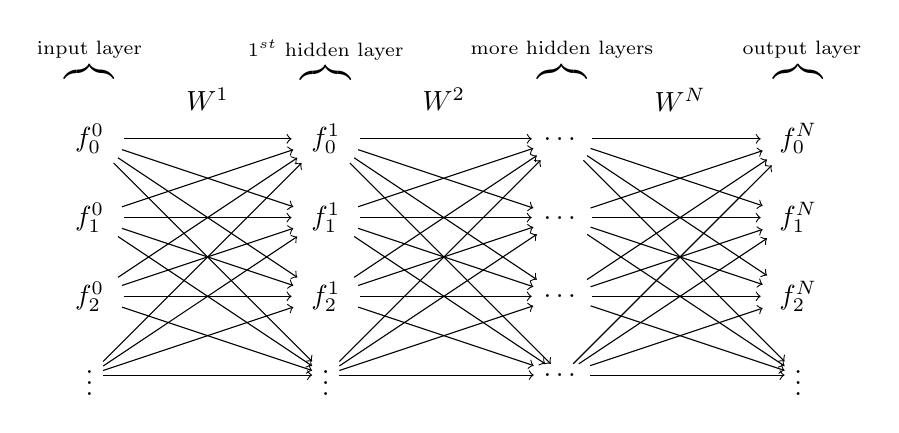
\begin{tikzpicture}
    % nodes
    \node         at (0,1)        {$\overbrace{}^{\text{input layer}}$};
    \node[circle] at (0,0)  (f00) {$f^0_0$};
    \node[circle] at (0,-1) (f01) {$f^0_1$};
    \node[circle] at (0,-2) (f02) {$f^0_2$};
    \node         at (0,-3) (f0)  {$\vdots$};
    \node         at (1.5,.5)(w1)  {$W^1$};

    \node         at (3,1)        {$\overbrace{}^{1^{st}\text{ hidden layer}}$};
    \node[circle] at (3,0)  (f10) {$f^1_0$};
    \node[circle] at (3,-1) (f11) {$f^1_1$};
    \node[circle] at (3,-2) (f12) {$f^1_2$};
    \node         at (3,-3) (f1)  {$\vdots$};
    \node         at (4.5,.5)(w2)  {$W^2$};

    \node         at (6,1)        {$\overbrace{}^\text{more hidden layers}$};
    \node[circle] at (6,0)  (f20) {$\dots$};
    \node[circle] at (6,-1) (f21) {$\dots$};
    \node[circle] at (6,-2) (f22) {$\dots$};
    \node         at (6,-3) (f2)  {$\dots$};
    \node         at (7.5,.5)(wN)  {$W^N$};

    \node         at (9,1)        {$\overbrace{}^{\text{ output layer}}$};
    \node[circle] at (9,0)  (fN0) {$f^N_0$};
    \node[circle] at (9,-1) (fN1) {$f^N_1$};
    \node[circle] at (9,-2) (fN2) {$f^N_2$};
    \node         at (9,-3) (fN)  {$\vdots$};

    % edges
    \path[->]
    % input layer
    (f00) edge (f10)
    (f00) edge (f11)
    (f00) edge (f12)
    (f00) edge (f1)

    (f01) edge (f10)
    (f01) edge (f11)
    (f01) edge (f12)
    (f01) edge (f1)

    (f02) edge (f10)
    (f02) edge (f11)
    (f02) edge (f12)
    (f02) edge (f1)

    (f0) edge (f10)
    (f0) edge (f11)
    (f0) edge (f12)
    (f0) edge (f1)
    % first hidden layer
    (f10) edge (f20)
    (f10) edge (f21)
    (f10) edge (f22)
    (f10) edge (f2)

    (f11) edge (f20)
    (f11) edge (f21)
    (f11) edge (f22)
    (f11) edge (f2)

    (f12) edge (f20)
    (f12) edge (f21)
    (f12) edge (f22)
    (f12) edge (f2)

    (f1) edge (f20)
    (f1) edge (f21)
    (f1) edge (f22)
    (f1) edge (f2)

    % output layer
    (f20) edge (fN0)
    (f20) edge (fN1)
    (f20) edge (fN2)
    (f20) edge (fN)

    (f21) edge (fN0)
    (f21) edge (fN1)
    (f21) edge (fN2)
    (f21) edge (fN)

    (f22) edge (fN0)
    (f22) edge (fN1)
    (f22) edge (fN2)
    (f22) edge (fN)

    (f2) edge (fN0)
    (f2) edge (fN1)
    (f2) edge (fN2)
    (f2) edge (fN)
    ;

  \end{tikzpicture}\end{center}
  Note that each layer can have a different \textit{width} (i.e. number of nodes in the layer). For each consecutive pair of layers $\pmb{f}^i,\pmb{f}^j$ (of widths $n_i,n_j$ respectively) there is an associated weight matrix $W\in\reals^{n_i\times n_j}$ st $\pmb{f}^j=W^T\pmb{f}^i$.
  \var The values from the output layer are then passed to an \textit{activation function} to make a classification. %TODO verify this
\end{definition}

\begin{remark}{Using MLPs}
  An MLP with a \textit{single} hidden layer is sufficient to represent any boolean or continuous function, althought the layer may be exponentially wider than the input.
  \par An MPL with \textit{two} hidden layers is sufficient to represent any mathematical function.
\end{remark}

\begin{proposition}{MLPs as Computation Graphs}
  \[\begin{array}{rrrll}
    &s_i^j&:=&(W^j)^Tf^{j-1}&\tiny \text{weighted sum of the }i^{th}\text{ node of the }j^{th}\text{ hidden layer}\\
    \implies&\dfrac{\partial s_i^j}{\partial w_{ii}^j}&=&f_i^{j-1}\\
    &f_i^j&:=&g_i^j(s_i^j)&\tiny i^{th}\text{ output vajue of }j^{th}\text{ hidden layer}\\
    \implies&\dfrac{\partial f_i^j}{\partial s_i^j}&=&\text{depends on def of }g_i^j
  \end{array}\]
\end{proposition}

\begin{proposition}{Output Layer for Classification Problem}
  To use an MLP for classification we require the output layer to represent a probability distribution for the possible classes (i.e. each node has a value in $[0,1]$ and the sum of all nodes is $1$).
  \par We can force outputs to reflect this distribution using a \textit{Softmax Neuron Group} in the last layer with activation function
  \[ g_j^N(s_j^N):=\frac{e^{s_j^N}}{\sum_{i\in\text{Group}\ e^{s_i^N}}} \]
  This has gradients
  \[\begin{array}{rcl}
    g'_j^N(s_j^N)&=&f_j^N(1-f_j^n)\\
    g'_j^N(s_{i\neq j}^N)&=&-f_j^Nf_i^N
  \end{array}\]
  All outputs $f_i^N:=g_i^N(s_i^N)$ range between 0 and 1, while the $\sum_{i\in\text{Group}}f_i=1$.
\end{proposition}

\subsection{Types of Deep Neural Networks}

\subsubsection{Fully Connected DNN}

%TODO

\subsubsection{Convolution DNN (CNNs)}

\begin{definition}{Convolution $*$}
  The \textit{Convolution} operation takes an input $x$ and a kernel $\omega$. The kernel is then applied to each element of the input. The actual operation depends on the set up of the input and the kernel (generally on their dimension).
  \[ (X*\omega)(i,j)=\sum_m\sum_nX_{i+m,j+n}\omega(m,n) \]
  The kernel is first placed st its the top-left entry overlaps the top-left entry of the input; the operation is applied; the kernel is then shifted right by one cell; this repeats until the right-side of the kernel surpasses the right-side of the input at which point is starts again but one cell lower. This means that $(X*\omega)$ is likely smaller in all dimensions that $X$.
  \begin{center}
    \includegraphics[width=.35\textwidth]{2dConvolution.PNG}
  \end{center}
\end{definition}

\begin{remark}{This is actually the Cross-Correlation operation, but is what is used in practice.}
  Convolution flips the kernel.
\end{remark}

\begin{definition}{Convolution DNN (CNNs)}
  \textit{Convoltuon DNN} expected an $n$-dimensional grid-like topology for its input (ie an $nD$-array of data). This means operations can be applied to individual or groups of cells and this \textit{CNNs} use \textit{convolution} in place of general matrix multiplication (in at least one of its layers). The kernels used by a CNN are typically $nD$-arrays of kernels (AKA a \textit{Tensor}) which are learnt from the data (rather than hand-crafted).
\end{definition}

\begin{remark}{Attraction of CNNs}
  CNNs have properties which distinguish them from Fully connected networks
  \begin{enumerate}
    \item \textit{Sparse Interactions}. In CNNs a node in one layer does not necessarily connected to every node in the next layer. This means that changing this node will not affect every node in the next layer. This is due to the grid structure of the input, where there is implicit relationships between adjacent cells/cell groups (e.g. adjacent pixels in an image). This means that nodes in later layers can have a greater \textit{receptive field of inputs}.
    \item \textit{Parameter Sharing}. The same parameter/weight is used for more than one function in the network. This can be considered as tying two parameters together st that have the same value. We use prior knowledge to decide which nodes to tie together (rather than doing it randomly). This reduces the number of parameters which need to be optimised (which means less data is required for training). The number of reduced parameters increases for later layers. This does not affect the runtime of the forward pass, but significantly reduces the memory requirements of the model.
    \item \textit{Equi-variant Representations}. If the input changes/shifts in a certain way (translation), then the output changes in exactly the same way. This is as a result of the previous two properties. However, CNNs are \underline{not} equivariant to rotation or scaling.
  \end{enumerate}
\end{remark}

\begin{definition}{Pooling Operation}
  A \textit{Pooling Operation} replaces the output of a network at a certain location with a summary of the outputs in nearby positions. This is applied after convolution and the activation function, and reduces the output size. \textit{Pooling} is typically similar to down sampling.
  \par \textit{Max Pooling} is a popular pooling operation where the output is changed to be the maximum value within a rectangular neighbourhood.
  \par Other pooling operations include: average pooling; weighted average pooling; $L^2$ norm etc.
\end{definition}

\begin{proposition}{Zero Padding}
  The \textit{kernel} shrinks the dataset, which we don't want as eventually the dataset would disappear. To avoid this \textit{Zero Padding} is used. \textit{Zero Padding} adds zeros to the outside of the input st the input and output are the same size after the kernel is applied to the original input data.
\end{proposition}

\begin{proposition}{Higher-Dimensional Data}
  When we have multiple data readings per instance (e.g. for each pixel of an RGB image) we consider each of these data fields to be a \textit{channel}. When we apply a convolution they must have the same dimension as the number of channels, and they can applied to both space \& channels. (ie a single convolution of an image is a 3D tensor). An extra dimension is added if we want to apply multiple filters/convolutions. The number of filters applied is equal to the number of channels in the next layer.
\end{proposition}

\begin{proof}{Convolution in Practice}
  In practice we do not convolve densely (ie every pixel), rather we skip certain pixels. The number of pixels skipped is referred to as the \textit{stride} of the layer. This results in downsampled convolutions.
\end{proof}

\begin{remark}{Care needs to be taken when backpropagating CNNs with zero padding or stride greater than 1.}\end{remark}

\begin{remark}{Typically CNNs start with convolution layers and then end with a couple of fully connected layers.}\end{remark}

\begin{remark}{Training CNNs}
  \begin{itemize}
    \item The most expensive part of training CNNs is training the convolutional layers. The fully-connected layers at the end are relatively inexpensive as they have a small number of features.
    \item When performing gradient descent, every gradient step requires a complete run of feed-forward propagation and backward propagation through the entire network.
  \end{itemize}
\end{remark}

\begin{proposition}{Residual Networks (ResNet)}
  \textit{ResNets} are a new innovation in CNNs where filters are applied to the input and then mergered back (by addition) with the input before be passed to the activation function. This leads to faster convergence by searching for weights which deviate only slightly from the identity. This allows for deeper networks.
  \begin{center}
    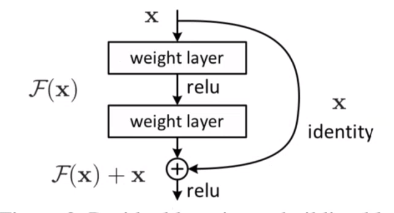
\includegraphics[width=.35\textwidth]{ResNet.PNG}
  \end{center}
\end{proposition}

\subsubsection{Recurrent DNN}

\subsection{Problems}

\subsubsection{Overfitting}

\begin{proposition}{High Parameter Space Overfitting}
  Multi-Layer perceptrons often have millions of neurons, with millions of parameters \& connections. These models have very high degrees of freedom and thus are prone to overfitting.
\end{proposition}

\begin{proposition}{Identifying Overfitting}
  When training a neural network we can plot the \textit{Loss Function} for the training data against that for the testing data, values after each epoch. Overfitting occurs if the distance between these lines increases over time.
  \begin{center}
    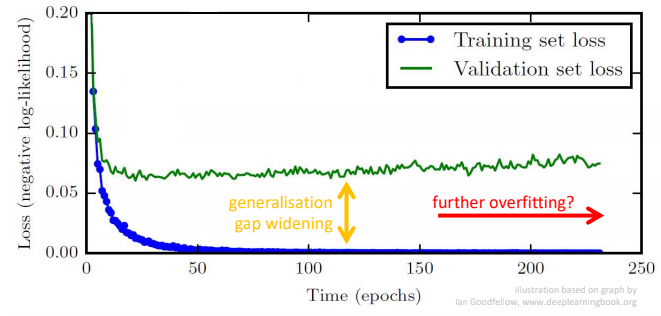
\includegraphics[width=.7\textwidth]{overfitting.PNG}
  \end{center}
  A natural idea from this is to keep a copy of the model with the smallest generalisation width, and then reverting to it after all the training.
\end{proposition}

\begin{remark}{Overfitting can always be addressed by using more data, more representative data and/or strategically sampling data.}
  Deep Learning techniques are particularly good at extract new information from new data. Whereas some older algorithms reach a ceiling where they can no longer learn form new information.
\end{remark}

\begin{proposition}{Obtaining More Data (Data Augmentation)}
  Data for deep learning is expensive to collect as it requires ground truth annotations. \textit{Data Augmentation} is a se of techniques used to increase the size of our data pool, without having to collect more data, by slightly modifying existing data. This can be done as an \textit{online process} during training.
  \par For images these techniques include: cropping, adding noise, rotating, translation, hue shift etc.
\end{proposition}

\begin{definition}{Regularisation}
  A \textit{Regularisation} is any modification made to a learning algorithm which is intended to reduced its \textit{generalisation error}, \underline{but} not its \textit{training error}.
\end{definition}

\begin{definition}{$L$-Regularisation}
  \textit{$L$-Regularisation} constrains the weight space (i.e. makes certain weight values more likely to be learned by the system).
\end{definition}

\begin{definition}{$L1$-Regularisation}
  \textit{$L1$-Regularisation} targets a local minimum with \textit{sparse} weights to combat overfitting (ie using very few nodes). This is done by introducing a penalty to the cost function for every weight, based on the \textit{absolute value} of the weight. This penalises non-zero weight values. This gives a cost function of the form
  \[ J(X;W)=\underbrace{\frac1{|X|}\sum_{x\in X}L(f(x;W),f^*(x))}_\text{normal cost function}+\frac12\sum_{w\in W}\mu|w| \]
  During training this gives us the update rule
  \[ W_{t+1}=W_t-\eta\cdot\left[\underbrace{\nabla J_\text{plain}(X;W^t)}_\text{normal cost function}+\mu\text{sign}(W^t)\right] \]
\end{definition}

\begin{definition}{$L2$-Regularisation}
  \textit{$L2$-Regularisation} targets a local minimum with \textit{small-magnitude} weights to combat overfitting (ie lots of nodes making small contributions). This is done by introducing a penalty to the cost function for every weight, based on the \textit{squared value} of the weight. This penalises higher weights more. This gives a cost function of the form
  \[ J(X;W)=\underbrace{\frac1{|X|}\sum_{x\in X}L(f(x;W),f^*(x))}_\text{normal cost function}+\frac12\sum_{w\in W}\lambda w^2 \]
  During training this gives us the update rule
  \[ W_{t+1}=W_t-\eta\cdot\left[\underbrace{\nabla J_\text{plain}(X;W^t)}_\text{normal cost function}+\lambda W^t\right] \]
\end{definition}

\begin{definition}{Dropout}
  \textit{Dropout} uses the idea that Neural Networks are in fact an ensemble of sub-networks (\texttt{Proposition 2.1}) and tries to define a training procedure so that each sub-network can learn (somewhat) independently by dropping out \underline{nodes}.
  \par This is done by, during each training loop, setting the incoming weights weights to a random set of nodes to 0 with probability $1-p$ (effectively immobilising a random set of neurons) and then training the network. This is particularly effective on fully connected networks.
  \par $p$ is often set to .5 before tuning on the validation set. During validation all weights are turned on, so the output of the network is significantly greater. To combat this weights are set to $pW$ in order to reduce their magnitude. $p$ is then tuned.
\end{definition}

\begin{definition}{DropConnect}
  \textit{DropConnect} is a variation on \textit{Dropout} where \underline{connections} are dropped, rather than nodes. This is done by setting a random set of weights to zero, with probability $1-p$, during each training cycle. This a more fine-grained approach to ensemble learning than \textit{Dropout}.
\end{definition}

\subsection{Usefulness}

\begin{remark}{Advantages of Deep Neural Networks}
  \begin{itemize}
    \item \textit{Hierarchical Automatic Modularisation}. A deep neural network has many layers, and the information of each layer is available to the succeeding layer. This means each layer can be considered to extract slightly more precise features (e.g. pixel colours $\to$ edges $\to$ corners $\to$ object parts $\to$ object class). These modular layers are generated automatically during training.
    \item \textit{Practical Performance}. Greater depth gives greater performance than greater width. Note that large networks require more training time and larger data sets.
    \item \textit{Oscillation Argument}. There are functions $f$ that can be represented by a \underline{deep} ReLU network with a polynomial number of neurons, whereas a \underline{shallow} network would require exponentially many units.
  \end{itemize}
\end{remark}

\subsection{Possible Extensions}

\begin{proposition}{Network Distillation}
  Is it possible to learn an ensemble of deep networks, but then \textit{compress} these deep networks into a single shallow (or more efficient) network? Sometimes.
\end{proposition}

\begin{proposition}{Mixture of Experts}
  We could learn a series of networks which each deal with a specific subtask of a problem and then use another network to decide which of these networks (or order of networks) to use in each instance.
\end{proposition}

\section{Training Algorithms}

\begin{definition}{Cost/Loss Function, $J$}
  A \textit{Cost Function} $J(\cdot;\cdot)$ is a real-valued measure of how inaccurate a classifier is for a given input configuration (test data \& weights). Greater values imply the classifier is less accurate. Here are some common cost functions
  \begin{itemize}
    \item[Expected Loss] $\displaystyle J(X;\pmb{w})=\expect[L(f(\pmb{x},\pmb{w}),f^*(\pmb{x}))]$
    \item[Empirical Risk] $\displaystyle J(X;\pmb{w})=\frac1{|X|}\sum_{\pmb{x}\in X}L(f(\pmb{x},\pmb{w}),f^*(\pmb{x}))$
  \end{itemize}
  Here $L(x,x^*)$ is a measure of loss (distance) between two values. This is defined by the user on a case by case basis. Popular definitions are: $|x-x^*|,\ (x-x^*)^2$ \& $\indexed\{x=x^*\}$
\end{definition}

\subsection{Gradient Descent}

\begin{definition}{Gradient Descent}
  \textit{Gradient Descent} aims to learn a set of weight values $\pmb{w}$ which produce a local minimum for a given cost function $J$. The update rule for gradient descent is
  \[ \pmb{w}_{t+1}=\pmb{w}_t-\underbrace{\eta\cdot\nabla J(X;\pmb{w}_t)}_{\Delta\pmb{w}} \]
  $\nabla J(X;\pmb{w}_t)$ is the partial derivative of the cost function wrt to the weights and gives the direction of the greatest descent. We can calculate the $i^\text{th}$ component of $\Delta\pmb{w}$ after observing $(\pmb{x},f^*(\pmb{x}))$
  \[ [\Delta\pmb{w}]_i=\eta x_i(\underbrace{\pmb{w}^T_t\pmb{x}}_{f(\pmb{x};\pmb{w}_t)}-f^*(\pmb{x})) \]
\end{definition}

\begin{definition}{Online Gradient Descent}
  \begin{enumerate}
    \item \texttt{initialise} all weights $W$ randomly.
    \item \texttt{for} $t=0,1,\dots$ \texttt{do}:
    \begin{enumerate}
      \item \texttt{pick} net training sample $(x,f^*)$.
      \item \texttt{forward-backward pass} to compute $\nabla J$.
      \item \texttt{update} weights $W\leftarrow W-\eta\nabla J$.
      \item \texttt{if} (stopping criteria met) \texttt{break loop}.
    \end{enumerate}
    \item \texttt{return} final weights $W$.
  \end{enumerate}
\end{definition}

\begin{remark}{Using Single Samples}
  Using single samples to find the minimum point of the cost function will only roughly approximate aspects of the cost function gradient in online mode, leading to a very noisy gradient descent which may not find the global minimum at all.
  \par Thus, it is not good to do online learning. And if the learning rate $\eta$ is set too \textit{large} then we may overshoot the global minimum. If the learning rate $\eta$ is set too \textit{small} then we takes a very long time to find a minimum.
\end{remark}

\begin{proposition}{Using Multiple Samples}
  As using a single sample is bad, we try using multiple samples at once and using the average $\nabla J$. There are two approaches
  \begin{itemize}
    \item \textit{Deterministic Gradient Descent} (DGD) where \underline{all} training samples $(X,F^*)$ are used. Given a small enough learning rate $\eta$ this will process to the true local minimum, but at high computational cost.
    \item \textit{Stochastic Gradient Descent} (MiniBatch) where a \underline{small subset} of training samples $(X,F^*)$ are used. This is still good at finding a minimum, and much less computationally costly.
  \end{itemize}
  For the average of $\nabla J$ we use
  \[ \nabla J=\frac1{|X|}\nabla_W\sum_j L(\underbrace{f(\mathbf{x}_j,W)}_\text{\tiny prediction},f^*) \]
\end{proposition}

\begin{proposition}{Setting the Learning Rate $\eta$}
  Setting the learning rate $\eta$ can be hard so a process called \textit{Simulated Annealing} is used to test out several learning rates.
  \par Let $\eta_0$ be an initial (high) learning rate and $\eta_\tau$ be a final (smaller) learning rate. \textit{Simulated Annealing} transitions from $\eta_0$ to $\eta_\tau$.
  \begin{enumerate}
    \item \texttt{initialise} all weights $W$ randomly.
    \item \texttt{for} $k=0,\dots,\tau$ \texttt{do}:
    \begin{enumerate}
      \item $\eta_k:=\left(1-\frac{k}\tau)\eta_0+\frac{k}\tau\eta_\tau$
      \item \texttt{for} $t=0,1,\dots$ \texttt{do}:
      \begin{enumerate}
        \item \texttt{pick} net training sample $(x,f^*)$.
        \item \texttt{forward-backward pass} to compute $\nabla J$.
        \item \texttt{update} weights $W\leftarrow W-\eta_k\nabla J$.
        \item \texttt{if} (stopping criteria met) \texttt{break loop}.
      \end{enumerate}
      \item \texttt{return} final weights $W$.
    \end{enumerate}
  \end{enumerate}
\end{proposition}

\subsubsection{Auto-Differentitation}

\begin{proposition}{Calculating Partial Derivatives}
  There are three ways to calculate the partial derivatives required for \textit{Gradient Descent}.
  \begin{itemize}
    \item \textit{Symbolic Differentiation} (i.e. algebra). Hard to define to work in all cases.
    \item \textit{Numerical Differentiation} (i.e. check values in a neighbourhood and approximate the best direction). Easy to implement but low accuracy and high computational cost.
    \item \textit{Automatic-Differentiation} using feedforward computation graphs. See below
  \end{itemize}
\end{proposition}

\begin{definition}{Feedforward Computational Graph}
  Given a series of equations we can construct a \textit{feedforward computational graph}. \textit{Feedforward computational graphs} have a node for each variable or constant, and then an edge between nodes which are dependent. Once values are defined for all variables at a given depth, values can easily be calculated for variables higher up the tree.
\end{definition}

\begin{example}{Feedforward Computational Graph}
  Consider the following series of equations
  \[\begin{array}{rclcrcl}
    a&=&b\times c&\quad&b&=&d+e\\
    c&=&e+2&&d&=&3+f\\
    e&=&f\times g
  \end{array}\]
  We can construct the following \textit{Computational Graph}
  \begin{center}\begin{tikzpicture}
    % nodes
    \node[circle] at (0,0)   (3) {$3$};
    \node[circle] at (0,-2)  (f) {$f$};
    \node[circle] at (0,-4)  (g) {$g$};

    \node[circle] at (2,-1)  (d) {$d=3+f$};
    \node[circle] at (2,-3)  (e) {$e=f\times g$};
    \node[circle] at (2,-5)  (2) {$2$};

    \node[circle] at (4,-2)  (b) {$b=d+e$};
    \node[circle] at (4,-4)  (c) {$c=e+2$};

    \node[circle] at (6,-3)  (a) {$a=b\times c$};

    % edges
    \path[->]
    (3) edge (d)
    (f) edge (d)
    (f) edge (e)
    (g) edge (e)

    (d) edge (b)
    (e) edge (b)
    (e) edge (c)
    (2) edge (c)

    (b) edge (a)
    (c) edge (a)
    ;
  \end{tikzpicture}\end{center}
\end{example}

\begin{proposition}{Feedforward Computational Graph - Neural Network}
  \begin{center}
    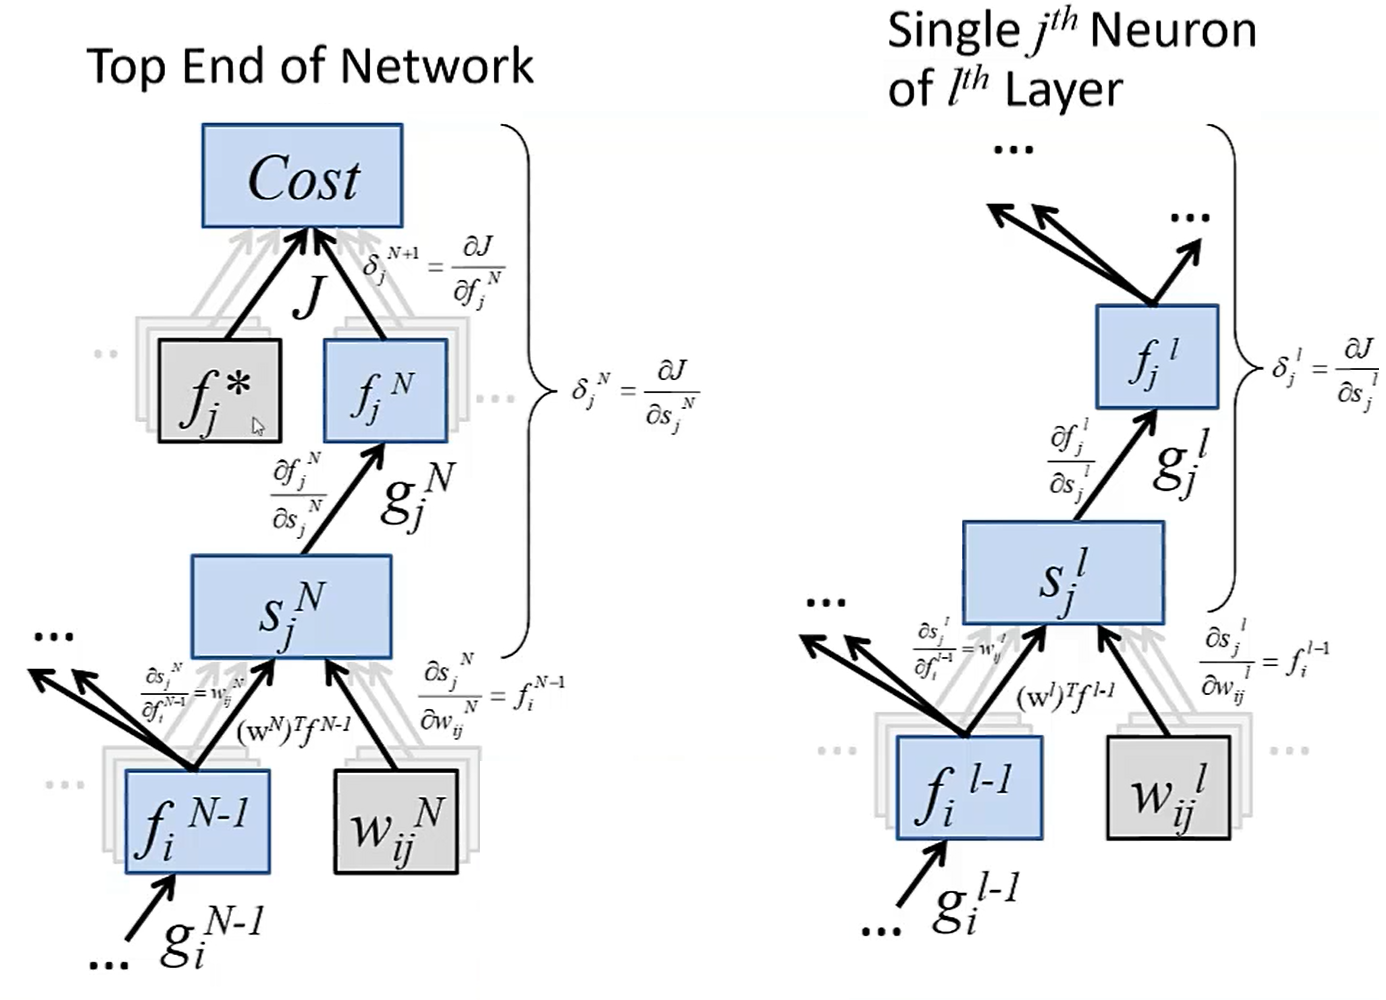
\includegraphics[width=.7\textwidth]{NeuralNetworkComputationalGraph.PNG}
  \end{center}
  Remember that $J(\cdot,\cdot)$ is the cost function; $s_j^l:=(w^l)^Tf^{l-1}$ is the signal of a layer; $g_j^l(\cdot)$ is the activation function of a layer; $f_j^l:=g_j^l(s_j^l)$ is the output of the layer;
\end{proposition}

\begin{definition}{Auto-Differentiation using a Feedforward Computational Graph}
  Consider two nodes in a computational graph $x,y$ and suppose you want to find the partial derivative $\frac{\partial x}{\partial y}$.
  \begin{enumerate}
    \item Establish all the paths from $y$ to $x$ in the graph.
    \item Calculate the partial derivatives of each step of these graphs. (i.e. if there is a path $y\to a\to x$ calculate $\frac{\partial a}{\partial y},\frac{\partial x}{\partial a}$).
    \item Apply the chain rule along each path (i.e. For $y\to a\to x$ calculate $\frac{\partial a}{\partial y}\cdot\frac{\partial x}{\partial a}$).
    \item Sum these calculations together to get the final result $\frac{\partial x}{\partial y}$.
    \item Substitute variables to make computation easier.
  \end{enumerate}
\end{definition}

\begin{example}{Auto-Differentiation using a Feedforward Computational Graph}
  Consider the graph in \texttt{Example 3.1} and wanting to calculate $\frac{\partial f}{\partial a}$.
  \begin{enumerate}
    \item There are three paths from $f$ to $a$ in the graph: (1) $f\to d\to b\to a$; (2) $f\to e\to b\to a$; and, (3) $f\to e\to c\to a$.
    \item We need to calculate the following partial derivatives: $\frac{\partial d}{\partial f},\frac{\partial b}{\partial d},\frac{\partial a}{\partial b}$ for (1); $\frac{\partial e}{\partial f},\frac{\partial b}{\partial e},\frac{\partial a}{\partial b}$ for (2); and, $\frac{\partial e}{\partial f},\frac{\partial c}{\partial e},\frac{\partial a}{\partial c}$ for (3).
    \[\begin{array}{rclcrclcrcl}
      &(1)&&&&(2)&&&&(3)\\
      \frac{\partial d}{\partial f}&=&1&\quad&\frac{\partial e}{\partial f}&=&g&\quad&\frac{\partial e}{\partial f}&=&g\\
      \frac{\partial b}{\partial d}&=&1&\quad&\frac{\partial b}{\partial e}&=&1&\quad&\frac{\partial c}{\partial e}&=&1\\
      \frac{\partial a}{\partial b}&=&c&\quad&\frac{\partial a}{\partial b}&=&c&\quad&\frac{\partial a}{\partial c}&=&b
    \end{array}\]
    \item Applying the chain rule to each path gives
    \[\begin{array}{rrcl}
      (1)&\frac{\partial d}{\partial f}\frac{\partial b}{\partial d}\frac{\partial a}{\partial b}&=&1\cdot1\cdot c=c\\
      (2)&\frac{\partial e}{\partial f}\frac{\partial e}{\partial f}\frac{\partial b}{\partial e}&=&g\cdot1\cdot1\cdot c=gc\\
      (3)&\frac{\partial e}{\partial f}\frac{\partial c}{\partial e}\frac{\partial a}{\partial c}&=&g\cdot1\cdot b=gb\\
    \end{array}\]
    \item Summing the terms together we get
    \[ \frac{\partial a}{\partial f}=c+gc+gb \]
    \item By substitution we get a final expression
    \[ \frac{\partial a}{\partial f}=2+5g+2fg+2fg^2 \]
  \end{enumerate}
  So when $f=4,g=2$ we have that $a=150$ and $\frac{\partial a}{\partial f}=60$.
\end{example}

\begin{proposition}{Using Hierarchical Dependency}
  By the chain rule we have that $\frac{\partial x}{\partial z}=\frac{\partial x}{\partial y}\frac{\partial y}{\partial z}$. So, if $\frac{\partial x}{\partial y}$ is already known then we just need to multiply that value by $\frac{\partial y}{\partial z}$ to get $\frac{\partial x}{\partial z}$.
  \par This can be utilised to ease the computational load of a calculation. In particular, calculating the derivatives one layer at a time is a good strategy.
\end{proposition}

\begin{remark}{Usefulness of Auto-Differentiation}
  \textit{Auto-Differentiation} allows us to mathematical quantify the affect one variable has on another, which is good. However, the number of paths in a network grows exponentially with the number of nodes, thus this can be computational hard. (\textit{Hierarchical Dependence} can be used to mitigate this)
\end{remark}

\subsection{Backpropagation Algorithm}

\begin{remark}{Backpropagation Algorithm - Intuition}
  The \textit{Backpropagation Algorithm} combines \textit{reverse auto-differentiation} with \textit{gradient descent}. Reverse auto-differentiation is used to find the relationship between the cost function and each weight; and gradient descent to perform stepwise adjustments on weights.
  \par The \textit{Backpropagation Algorithm} seeks to compute the discrepancy between the network's output and the target value; then propagate this discrepancy backwards through the network to determine the influence of each weight on this discrepancy, by considering the influence of each path.
\end{remark}

\begin{proposition}{Backpropagation Algorithm - Overall Strategy}
  \begin{enumerate}
    \item Read the input \& perform a forward pass through the network. (This will calculate all $s_j^l,f_j^l$.)
    \item Calculate the cost function between each final layer neuron and its target $J(f_j^*,f_j^N)$.
    \item Calculate the error derivatives $\delta_j^{N+1}$ of the cost function $J$ wrt each final layer neuron $f_j^N$
    \[ \delta_j^{N+1}:=\frac{\partial J}{\partial f_j^N} \]
    \item Compute the error derivative $\delta_j^N$ of the cost function wrt the signals of the last layer
    \[ \delta_j^N:=\frac{\partial J}{\partial s_j^N}=g_j^N'(s_j^N)\cdot\delta_j^{N+1} \]
    \item Layer-by-layer calculate the \textit{error derivatives} $\delta_i^{l-1}$ of the cost function wrt the signal each neuron in the next layer, using the error derivatives $\delta_j^l$ of the layer above
    \[ \delta_i^{l-1}:=\frac{\partial J}{\partial s_i^{l-1}}=g_i^{l-1}'(s_i^{l-1})\sum_{j=1}^{d(l)}w_{ij}^l\delta_j^l \]
    \item Calculate the error derivates wrt to the weights of each neuron $\frac{\partial J}{\partial w_{ik}^l}$ using the error derivatives of the neuron activities $\delta_j^l$.
    \[ \frac{\partial J}{\partial w_{ij}^l}=\frac{\partial J}{\partial s_j^l}\frac{\partial s_j^l}{\partial w_{ij}^l}=\delta_j^lf_i^{l-1} \]
  \end{enumerate}
\end{proposition}

\begin{proof}{Derivation of $\delta_i^{l-1}$}
  \[\begin{array}{rrl}
    \delta_i^{l-1}&:=&\frac{\partial J}{\partial s_i^{l-1}}\\
    &=&\displaystyle\sum_{j=1}^{d(l)}\underbrace{\frac{\partial J}{\partial s_j^l}}_{\delta_j^l} \underbrace{\frac{\partial s_j^l}{\partial f_j^{l-1}}}_{w_{ij}^l} \underbrace{\frac{\partial f_i^{l-1}}{\partial s_i^{l-1}}}_{g^{l-1}_i'(s_i^{l-1})}\\
    &=&\displaystyle\sum_{j=1}^{d(l)}\delta_j^lw_{ij}^lg_i^{l-1}'(s_i^{l-1})\\
    &=&\displaystyle g_i^{l-1}'(s_i^{l-1})\sum_{j=1}^{d(l)}w_{ij}^l\delta_j^l
    \end{array}\]
\end{proof}

\begin{proposition}{Backpropagation Algorithm}
  \begin{enumerate}
    \item \texttt{initialise} all weights randomly (typically to small values).
    \item \texttt{for} $t=0$ \texttt{do}
    \begin{enumerate}
      \item \texttt{pick} next training sample $([f_1^0,f_2^0,\dots],[f_1^*,f_2^*,\dots])$.
      \item \texttt{forward pass} compute all layer outputs $\displaystyle s_j^l:=\sum_{i=1}^{d(l-1)}w_{ij}^lf_i^{l-1}$ and $\displaystyle f_j^l:=g_j^l(s_j^l)$. [i)]
      \item \texttt{compute} derivative of cost function wrt final layer $\delta_j^N:=g_j^N'(s_j^N)\cdot \frac{\partial J}{\partial f_j^N}$. [ii)-iii)]
      \item \texttt{backward pass} compute all deltas $\delta_i^{l-1}:=\displaystyle g_i^{l-1}'(s_i^{l-1})\sum_{j=1}^{d(l)}w_{ij}^l\delta_j^l$ [iv)-vi)]
      \item \texttt{update} all weights based on deltas and neuron activities $w_{ij}^l\leftarrow w_{ij}^l-\eta f_i^{l-1}\delta_j^l$ [gradient descent]
      \item \texttt{if} (stopping criteria met): \texttt{break loop}
    \end{enumerate}
    \item \texttt{return} final weights $w_{ij}^l$
  \end{enumerate}
\end{proposition}

\begin{remark}{Issues with Backpropagation Algorithm}
  The \textit{Backpropagation Algorithm} was known for 30 years before deep learning began. There are a few factors which prevented deep learning starting earlier:
  \begin{itemize}
    \item The \textit{Vanishing Gradient Problem}. Gradients are unstable/noisey when you backpropagate gradients in a very deep network.
    \item Descent-based optimisation techniques need to work accurately and \underline{fast in practice}, despite large training data sets. This was not possible before GPU parallelisation and improved optimisers.
    \item The number of parameters explode in deep networks (every node in one layer is connected to every node in the next layer, for all layers!). This can be addressed by sharing parameters (e.g. CNNs) or reuse parameters (e.g. RNNs).
    \item Regularisation techniques are critical to achieve good generalisation beyond the training data available (avoid overfitting).
  \end{itemize}
\end{remark}

\begin{remark}{Activation Functions need to be Differentiable \& Non-Linear}
  For the \textit{Back-Propagation Algorithm} the derivative of each activation function is used, so each activation function must be differentiable.
  \par The step-function does not fulfil this. $\tanh$ was consider as an alternative, however the gradient of its derivative is vanishingly small on the tails. This causes $\delta_i^{l-1}$ to become close to 0 (are saturated), significantly slowing down learning of early layers (if any learning occurs at all).
  \par This is addressed (usually) by forwarding signal via a residual neural network (ResNet), or using specially robust neuron layouts.
\end{remark}

\begin{definition}{Rectifying Linear Unit (ReLU)}
  \textit{ReLU} is an activation function which combines high speed of evaluation with a non-saturating non-linear function
  \[\begin{array}{rcl}
      g_{ReLU}(s)&:=&\max\{0,s\}\\
      g_{ReLU}'(s)&:=&\begin{cases}1&\text{if }s\geq0\\0&\text{otherwise}\end{cases}
  \end{array}\]
\end{definition}

\begin{remark}{Usefulness of ReLU}
  Using \textit{ReLU} may reach network convergence 5-10 times faster than using $\tanh$.
  \par However, using \textit{ReLU} introduces a problem of \textit{Dying Neurons} where a large gradient flowing through \textit{ReLU} may force the neuron never to activate again (as it pushes the incoming signal to 0). This is bad, as these neurons will no longer contribute to learning anymore.
\end{remark}

\subsection{Momentum}

\begin{proposition}{Learning via Momentum}
  Learning via \textit{Momentum} is an extension of gradient descent. A velocity term $v$ for \textit{`current descent speed`} is introduce. The velocity term defines the step sizes, depending upon how large \& how aligned to previous gradients a new gradient is.
  \par Formally we now define weight updates as
  \[ W_{t+1}=W_t+\underbrace{v_{t+1}}_\text{\tiny momentum}\quad\text{where}\quad v_{t+1}=\underbrace{\alpha}_{ \underset{\text{parameter}}{\text{momentum}}}\cdot v_t-\eta\nabla J(X;W_t) \]
  Momentum can overshoot.
\end{proposition}

\begin{proposition}{Nesterov Accelerated Gradient (NAG)}
  \textit{Nesterov Accelerated Gradient} is an extension of \textit{Learning via Momentum}, where instead of calculating the gradient at the current position you lookahead at the gradient of the target. This is since \textit{Momentum} will carry us towards the next location anyway.
  \par Formally we now define weight updates as
  \[ W_{t+1}=W_t+v_{t+1}\quad\text{where}\quad v_{t+1}=\alpha v_t-\eta\nabla J(X;\underbrace{W_t+\alpha v_t}_{ \underset{\text{perview}}{\text{location}}}) \]
  NAG is consistently better that \textit{Learning via Momentum} in practice.
\end{proposition}

\begin{remark}{When Momentum Struggles}
  Methods which use momentum progress very slowly in shallow plateau regions of the cost function state space as momentum is not able to build up.
  \par This can be rectified by improving the learning rate.
\end{remark}

\begin{proposition}{Newton's Method}
  \textit{Newton's Method} removes all hyperparameters (inc. \textit{Learning Rate} $\eta$) and instead uses curvature to rescale the gradient, by multiplying the gradient by the inverse Hessian of the current cost function $H(J(X;W_t))$. This leads to an optimisation that takes aggressive steps in directions of shallow curvature, and shorter steps in directions of steep curvature.
  \par Formally we now define weight updates as
  \[ W_{t+1}=W_t- H(J(X;W_t))^_{-1}\nablda J(X;W_t)\]
  \par Computing and inverting the Hessian is computationally and space expensive. Newton's method is attracted to saddle points (bad!).
\end{proposition}

\begin{remark}{The more parameters there are the more likely saddle points are}
  Saddle points occur when the hessian has both positive \& negative eigenvalues. This is more likely when we have more parameters (as the probability of all eigenvalues being positive is low).
  \par Random Matrix Theory states that the lower the cost function $J$ is (ie the closer it is to the global minimum), the more likely to find positive eigenvalues. This means that if we find a minimum it is likely to be a good one (i.e. low cost).
  \par Thus, most critical points with higher cost values $J$ should be saddle points, which we can escape using symmetry-breaking descent methods.
\end{remark}

\subsection{Function Adaptive Optimisation Algorithms}

\begin{definition}{Adaptive Gradient Algorithm (AdaGrad)}
  The \textit{AdaGrad} algorithm keeps track of per-weight learning rates to force evenly spread learning speeds across the weights. This means that weights with a high gradient have their learning rate decreases, whilst those with low gradients have it increased.
  \par Formally we now define weight updates as
  \[
    W_{t+1}=W_t-\eta\dfrac{\nabla J(X;W_t)}{\sqrt{A_{t+1}+\varepsilon}}\quad\text{where}\quad A_{t+1}=A_t+\big(\nabla J(X;W_t)\big)^2
  \]
  NOTE perform element-by-element squaring and $\varepsilon$ is used to avoid division by zero.\\
  $A_t$ is an accumulator vector, which accumulates the changes so far in each dimension.
\end{definition}

\begin{remark}{Limitations of Monotonic Learning}
  \textit{Monotonic Learning} is very aggressive and lacks the possibility of late adjustments, meaning learning usually stops too early.
\end{remark}

\begin{proposition}{Root-Mean-Square Propagation (RMSProp)}
  \textit{RMSProp} combats the aggressive reduction in \textit{AdaGrad}'s learning speed by propagation of a smooth running average, using a smoothing parameter $\beta$.
  \par Formally we now define weight updates as
  \[
    W_{t+1}=W_t-\eta\dfrac{\nabla J(X;W_t)}{\sqrt{A_{t+1}+\varepsilon}}\quad\text{where}\quad A_{t+1}=\beta A_t+(1-\beta)\big(\nabla J(X;W_t)\big)^2
  \]
  NOTE perform element-by-element squaring and $\varepsilon$ is used to avoid division by zero.\\
\end{proposition}

\begin{proposition}{Adaptive Moment Estimation (AdaM)}
  The \textit{AdaM} algorithm is an extension of \textit{RMSProp} with two new additions.
  \begin{enumerate}
    \item Smoothing \textit{RMSProp's} (usually noisy) incoming gradient by using a new parameter $\alpha$
    \item Correcting the impact of bias which is introuced by \textit{initialising} the two smoother measures.
  \end{enumerate}
  \[\begin{array}{rcl}
    G_{t+1}&=&\alpha G_t+(1-\alpha)\nabla J(X;W_t)\\
    \bar{G}&=&\dfrac{G_{t+1}}{1-\alpha^t}\\
    A_{t+1}&=&\beta A_t+(1-\beta)[\nabla J(X;W_t)]^2\\
    \bar{A}&=&\dfrac{A_{t+1}}{1-\beta^t}\\
    W_{t+1}&=&W_t-\eta\dfrac{\bar{G}_{t+1}}{\sqrt{\bar{A}_{t+1}}+\varpepsilon}
  \end{array}\]
\end{proposition}

\begin{remark}{Using AdaM}
  Applying AdaM to a ReLU-based network is sufficient to perform deep learning but there is no guarantee of success for a few reasons
  \begin{enumerate}
    \item We have hyperparameters $\alpha,\beta,\varepsilon,\dots$ which need to be set
    \item The size of each mini-batch is not certain.
    \item How do we initialise the network?
    \item How do we avoid overfitting? Especially with so many parameters.
    \item Which loss function to use.
  \end{enumerate}
  Achieving top-end results in deep learning often involves lots of parameter tuning, testing and trial-and-error.
\end{remark}

\subsection{Cost Functions for Classification}

\begin{remark}{Cost Functions for Classification Problem}
  In classification problems it is not obvious how to define the distance between classifications, and thus how to define a cost function. Using the setup of activation functions proposed in \texttt{Proposition 2.5} it is common to use the \textit{Cross-Entropy Cost Function}
\end{remark}

\begin{definition}{Cross-Entropy Cost Function}
  Let $f^*_j$ be the ground truth for output node $j$ and $f_j^N$ be our predicted value for the ground truth for output node $j$. The \textit{Cross-Entropy Cost Function} is define as
  \[\begin{array}{rrl}
  J&=&-\displaystyle\sum_{j\in\text{Group}}f_j^*\ln(f_j^N)\\
  \delta_i^N&=&\displaystyle\sum_{j\in\text{Group}}\frac{\partial J}{\partial f_j^N}\frac{\partial f_j^N}{\partial s_i^N}\\
  &=&f_i^N-f_i^*
  \end{array}\]
  The steepness of the cost function derivative $\frac{\partial J}{\partial f_j^N}$ \underline{exactly} cancels the shallowness of the softmax derivative $\frac{\partial f_j^N}{\partial s_i^N}$, leading to an \textit{MSE-Style Delta} $\delta+i^N$ which is propagated backwards from layer $N$.
\end{definition}

\begin{proposition}{Derivation of $\delta_i^N$ for Cross-Entropy Cost Function}
  \everymath={\displaystyle}
  \[\begin{array}{rrlcl}
    \delta_i^N&:=&\frac{\partial J}{\partial s_i^N}&\quad&\\
    &=&-\sum_{j\in\text{Group}}f_j^*\underbrace{\frac{\partial \ln(f_j^N)}{\partial s_i^N}}_\text{apply chain rule}\\
    &=&-\sum_{j\in\text{Group}}f_j^*\frac1{f_j^N}\frac{\partial f_j^N}{\partial s_i^N}&&\text{where }f_j^N:=\frac{e^{s_j^N}}{\sum_{i\in\text{Group}e^{s_i^N}}}\\
    &=&-\sum_{j=i}f_j^*\frac1{f_j^N}\underbrace{f_j^N(1-f_j^N)}_{\frac{\partial f_j^N}{\partial s_i^N}\text{ for }i=j}-\sum_{j\neq i}f_j^*\frac1{f_j^N}\underbrace{(-f_j^Nf_i^N)}_{\frac{\partial f_j^N}{\partial s_i^N}\text{ for }i\neq j}\\
    &=&-f_i^*(1-f_i^N)+\sum_{j\neq i}f_j^*\frac{f_j^Nf_i^N}{f_j^N}\\
    &=&-f_i^*+\underbrace{f_i^*f_i^N+\sum_{j\neq i}f_j^*f_i^N}_{=f_i^N\sum_{j\in\text{Group}}f_j^*}\\
    &=&f_i^N\underbrace{\left(\sum_{j\in\text{Group}}f_j^*\right)}_{=1}-f_i^*\\
    &=&f_i^N-f_i^*
  \end{array}\]
\end{proposition}

\section{Implementation}

\begin{remark}{Tuning}
  When tuning hyper-parameters we want to maximise test accuracy (not training accuracy) and minimise computational load (ie how long the execution takes)
\end{remark}

\begin{proposition}{Order of Hyper-parameter Tuning}
  \begin{enumerate}
    \item Learning Rate
    \item Batch Size
  \end{enumerate}
\end{proposition}

\begin{remark}{Learning Rate}
  When tuning the \textit{Learning Rate} there is a trade-off between speed (not too small) and actually converging (not too big).
\end{remark}

\begin{remark}{Batch Size}
  \textit{Batch Size} is the number of examples propagated through the network at any one time. The risk with smaller batch sizes is that they do not sufficiently represent the entire dataset, so the parameter updates overfit to that batch. The risk with larger batch sizes result in fewer weight updates as fewer epochs are completed
  \par Larger batch sizes generally make the execution quicker, due to few passes being completed. Smaller batches are better able to utilise a GPU's parallel processing capability.
\end{remark}

\begin{definition}{Batch Normalisation}
  \textit{Batch Normalisation} normalises layer inputs so the distribution of these inputs does not vary while training and adjusting parameters. This speeds up convergence by changing each input distribution to have zero mean and unit variance. The equation used is
  \[ \hat{x}_{i,c,x,y}=\frac{x_{i,c,x,y}-\mu_c}{\sqrt{\sigma^2_c+\epsilon}} \]
  where $x_{i,c,x,y}$ is an output from the previous layer, $\hat{x}_{i,c,x,y}$ is the transformed value which will be used as an input, $i,c,x,y$ define the batch,channel,width \& height position of the input, $\mu_c$ and $\sigma^2_c$ are the mean and variance for each training batch; $\epsilon$ is a small constant for numerical stability (ie when $\sigma^2_c$ is 0).
  \par \textit{Batch Normalisation} limits the functions a neural network can represent (bad!). To restore this representation power we learn two new parameters per channel $\gamma_c$ and $\beta_c$. Giving
  \[ \hat{x}_{i,c,x,y}=\gamma_c\cdot\frac{x_{i,c,x,y}-\mu_c}{\sqrt{\sigma^2_c+\epsilon}}+\beta_c \]
  \textit{Batch Normalisation} is typically added after each convolution or fully connected layer, and before the activation function.
\end{definition}

\begin{remark}{Other Ways to Optimise}
  Momentum can be added to SGD. This adds another hyper-parameter to be tuned.
\end{remark}

\newpage
\setcounter{section}{-1}
\section{Reference}

\begin{definition}{Hessian Matrix}
  \[ H(J)=\begin{pmatrix}\frac{\partial J^2}{\partial w_1^2}&\frac{\partial J^2}{\partial w_1\partial w_2}&\dots&\frac{\partial J^2}{\partial w_1\partial w_n}\\\frac{\partial J^2}{\partial w_2\partial w_1}&\frac{\partial J^2}{\partial w_2^2}&\dots&\frac{\partial J^2}{\partial w_2\partial w_n}\\\vdots&\vdots&\ddots&\vdots\\\frac{\partial J^2}{\partial w_n\partla w_1}&\frac{\partial J^2}{\partial w_n\partial w_2}&\dots&\frac{\partial J^2}{\partial w_n^2}\end{pmatrix}\]
\end{definition}

\end{document}
